\section{Why study generative modeling?}
\label{sec:why}

One might legitimately wonder why generative models are worth studying,
especially generative models that are only capable of generating data
rather than providing an estimate of the density function.
After all, when applied to images, such models seem to merely provide
more images, and the world has no shortage of images.

There are several reasons to study generative models, including:
\begin{itemize}

\item Training and sampling from generative models is an excellent test
of our ability to represent and manipulate high-dimensional probability
distributions.
High-dimensional probability distributions are important objects in a
wide variety of applied math and engineering domains.

\item Generative models can be incorporated into reinforcement learning in several
  ways.
  Reinforcement learning algorithms can be divided into two categories;
  model-based and model-free, with model-based algorithms being those that
  contain a generative model.
  Generative models of time-series data can be used to simulate possible
futures. Such models could be used for planning and for reinforcement learning
in a variety of ways.
A generative model used for planning can learn a conditional distribution over
future states of the world, given the current state of the world and hypothetical
actions an agent might take as input.
The agent can query the model with different potential actions and choose actions
that the model predicts are likely to yield a desired state of the world.
For a recent example of such a model, see \citet{finn2016unsupervised},
and for a recent example of the use of such a model for planning,
see \citet{finn2016deep}. 
Another way that generative models might be used for reinforcement learning is
to enable learning in an imaginary environment, where mistaken actions do not
cause real damage to the agent.
Generative models can also be used to guide exploration by keeping track of
how often different states have been visited or different actions have been
attempted previously.
Generative models, and especially GANs, can also be used for inverse reinforcement
learning.
Some of these connections to reinforcement learning are described further in
\secref{sec:rl_connections}.

\item Generative models can be trained with missing data and can provide predictions
  on inputs that are missing data.
  One particularly interesting case of missing data is {\em semi-supervised learning},
  in which the labels for many or even most training examples are missing.
  Modern deep learning algorithms typically require extremely many labeled examples
  to be able to generalize well.
  Semi-supervised learning is one strategy for reducing the number of labels.
  The learning algorithm can improve its generalization by studying a large number
  of unlabeled examples which, which are usually easier to obtain.
  Generative models, and GANs in particular, are able to perform semi-supervised
  learning reasonably well. This is described further in \secref{sec:ssl}.

\item Generative models, and GANs in particular, enable machine learning to work with
  {\em multi-modal} outputs.
  For many tasks, a single input may correspond to many different correct answers,
  each of which is acceptable.
Some traditional means of training machine learning models, such as minimizing the
mean squared error between a desired output and the model's predicted output, are
not able to train models that can produce multiple different correct answers.
One example of such a scenario is predicting the next frame in a video, as shown
in \figref{fig:lotter}.

\item Finally, many tasks intrinsically require realitic generation of samples from
  some distribution.
\end{itemize}

\begin{figure}
\centering
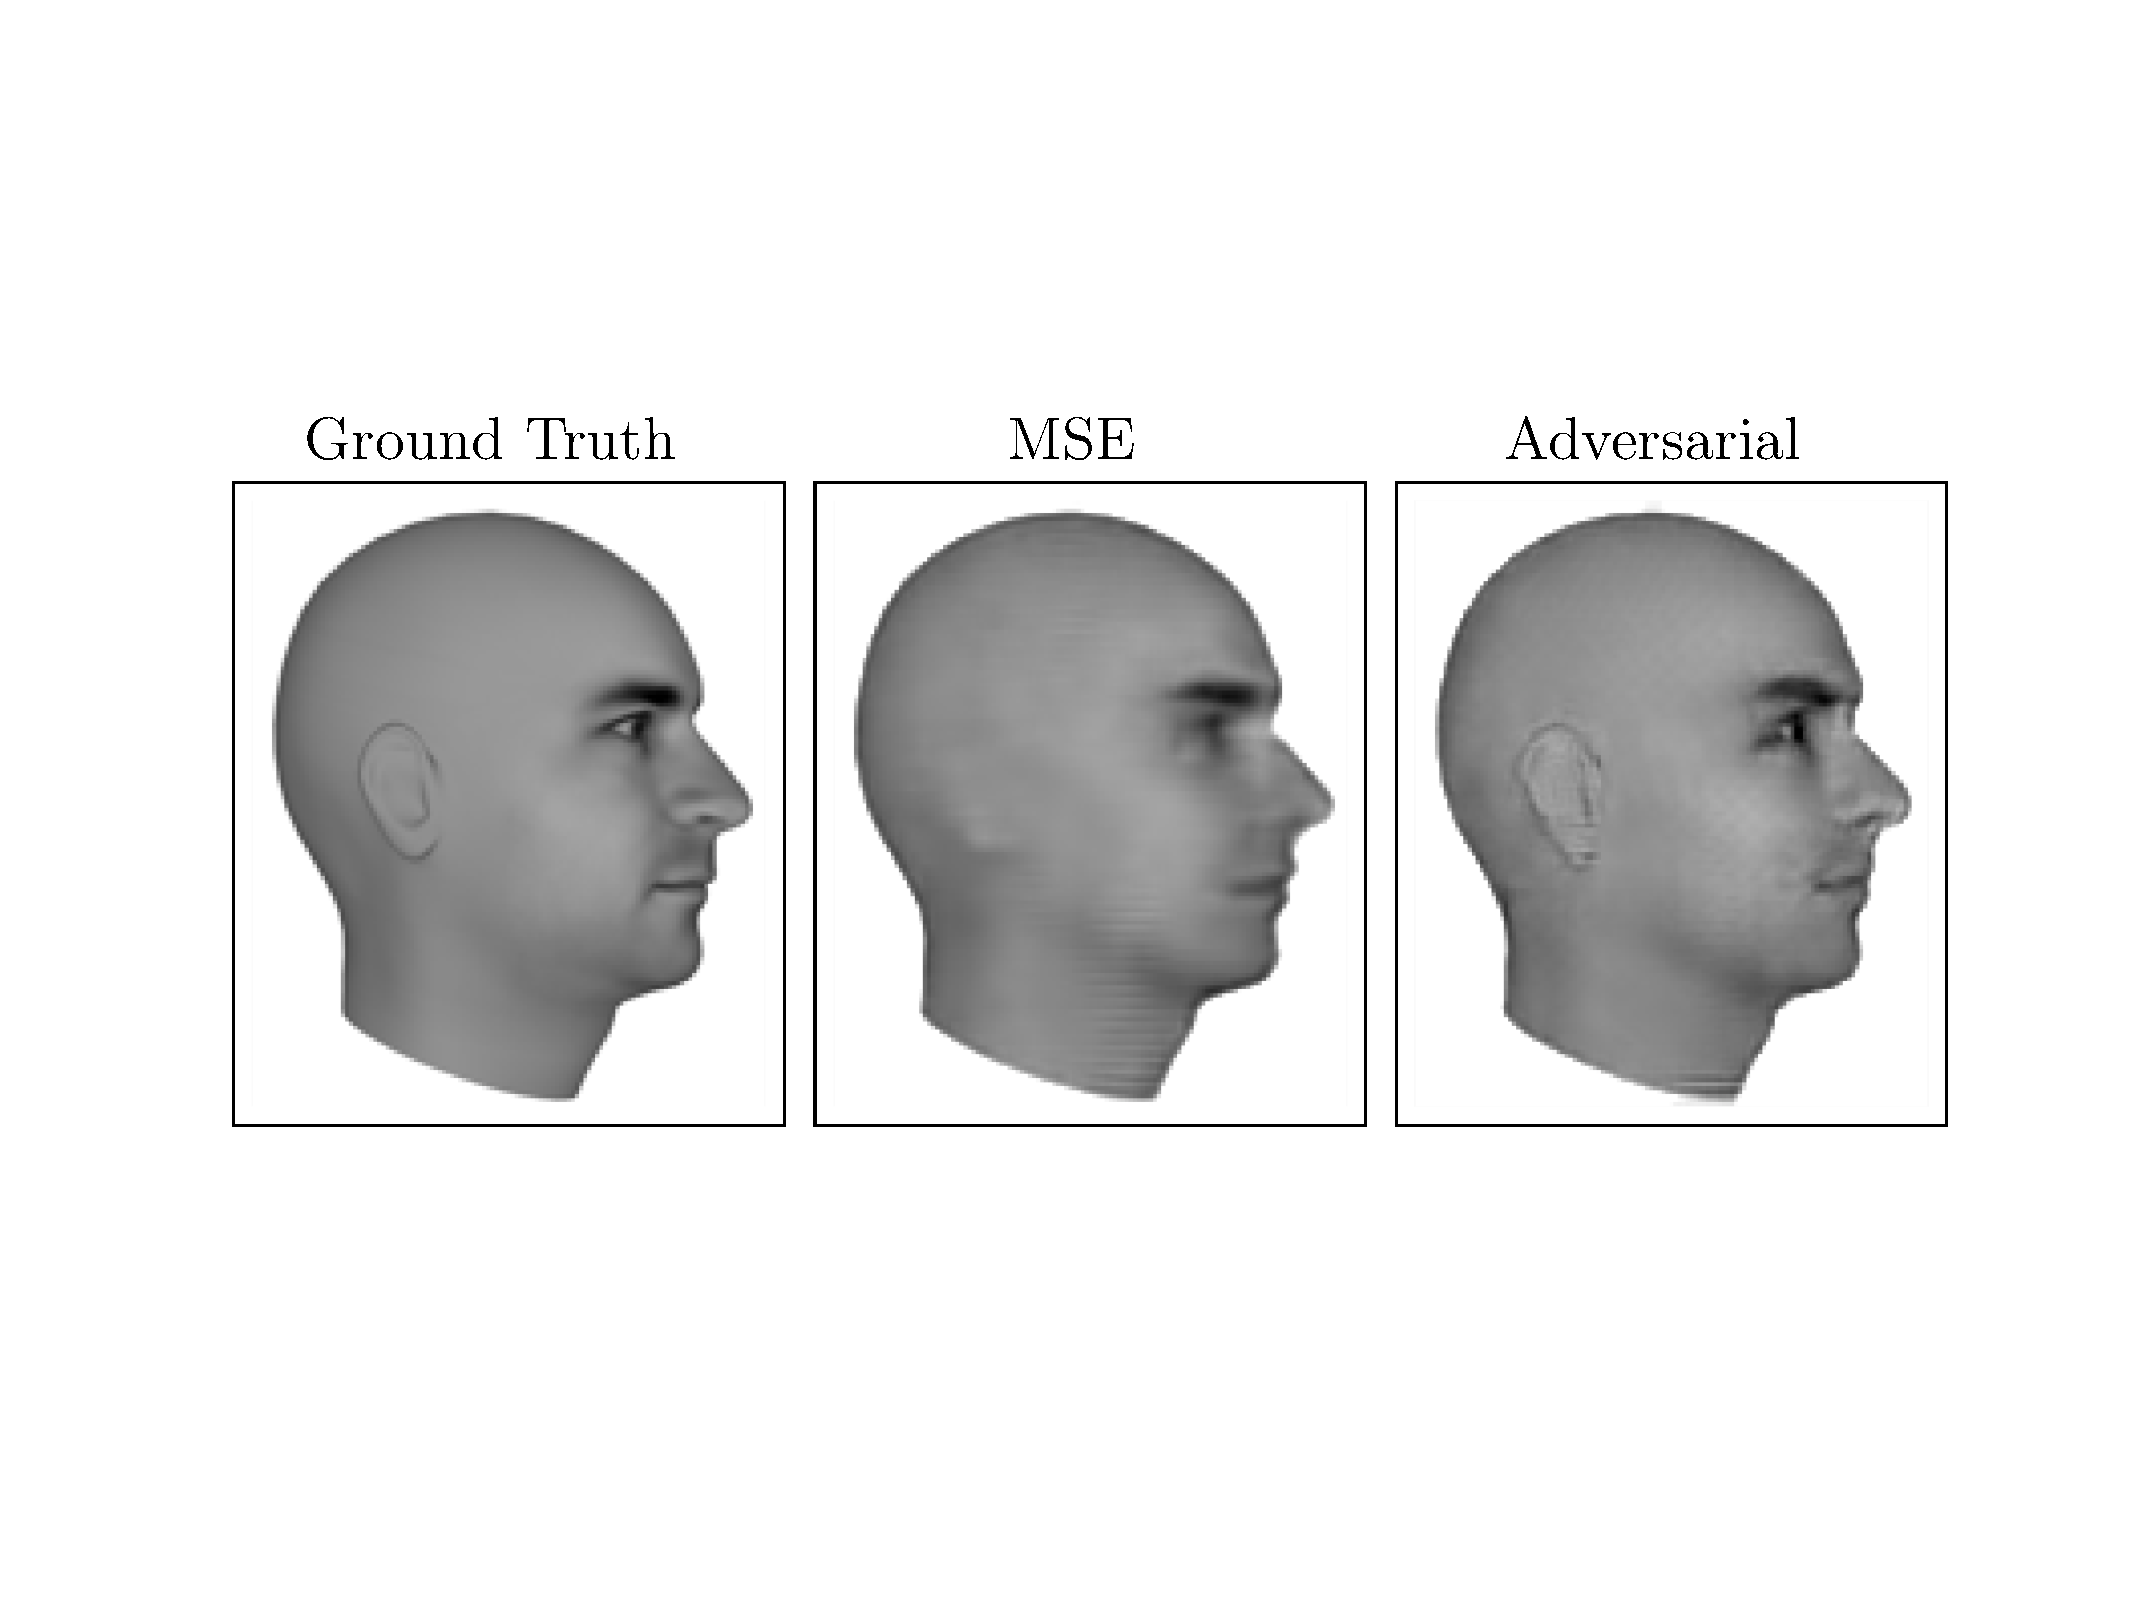
\includegraphics[width=\textwidth]{lotter.pdf}
\caption{
\citet{lotter2015unsupervised} provide an excellent illustration of the importance
of being able to model multi-modal data.
In this example, a model is trained to predict the next frame in a video sequence.
The video depicts a computer rendering of a moving 3D model of a person's head.
The image on the left shows an example of an actual frame of video, which the model
would ideally predict.
The image in the center shows what happens when the model is trained using mean
squared error between the actual next frame and the model's predicted next frame.
The model is forced to choose a single answer for what the next frame will look like.
Because there are many possible futures, corresponding to slightly different positions
of the head, the single answer that the model chooses corresponds to an average over
many slightly different images.
This causes the ears to practically vanish and the eyes to become blurry.
Using an additional GAN loss, the image on the right is able to understand that there
are many possible outputs, each of which is sharp and recognizable as a realistic,
detailed image.
}
  \label{fig:lotter}
\end{figure}

Examples of some of these tasks that intrinsically require the generation of good
samples include:
\begin{itemize}
  \item {\em Single image super-resolution}: In this task, the goal is to take a
    low-resolution image and synthesize a high-resolution equivalent.
    Generative modeling is required because this task requires the model to impute
    more information into the image than was originally there in the input.
    There are many possible high-resolution images corresponding to the low-resolution
    image.
    The model should choose an image that is a sample from the probability distribution
    over possible images.
    Choosing an image that is the average of all possible images would yield a result
    that is too blurry to be pleasing.
    See \figref{fig:superres}.

  \item Tasks where the goal is to create art.
    Two recent projects have both demonstrated that generative models, and in particular,
    GANs, can be used to create interactive programs that assist the user in creating
    realistic images that correspond to rough scenes in the user's imagination.
    See \figref{fig:igan} and \figref{fig:ian}.

  \item Image-to-image translation applications can convert aerial photos into maps
    or convert sketches to images. There is a very long tail of creative applications
    that are difficult to anticipate but useful once they have been discovered.
    See \figref{fig:im2im}.

\end{itemize}

\begin{figure}
  \centering
  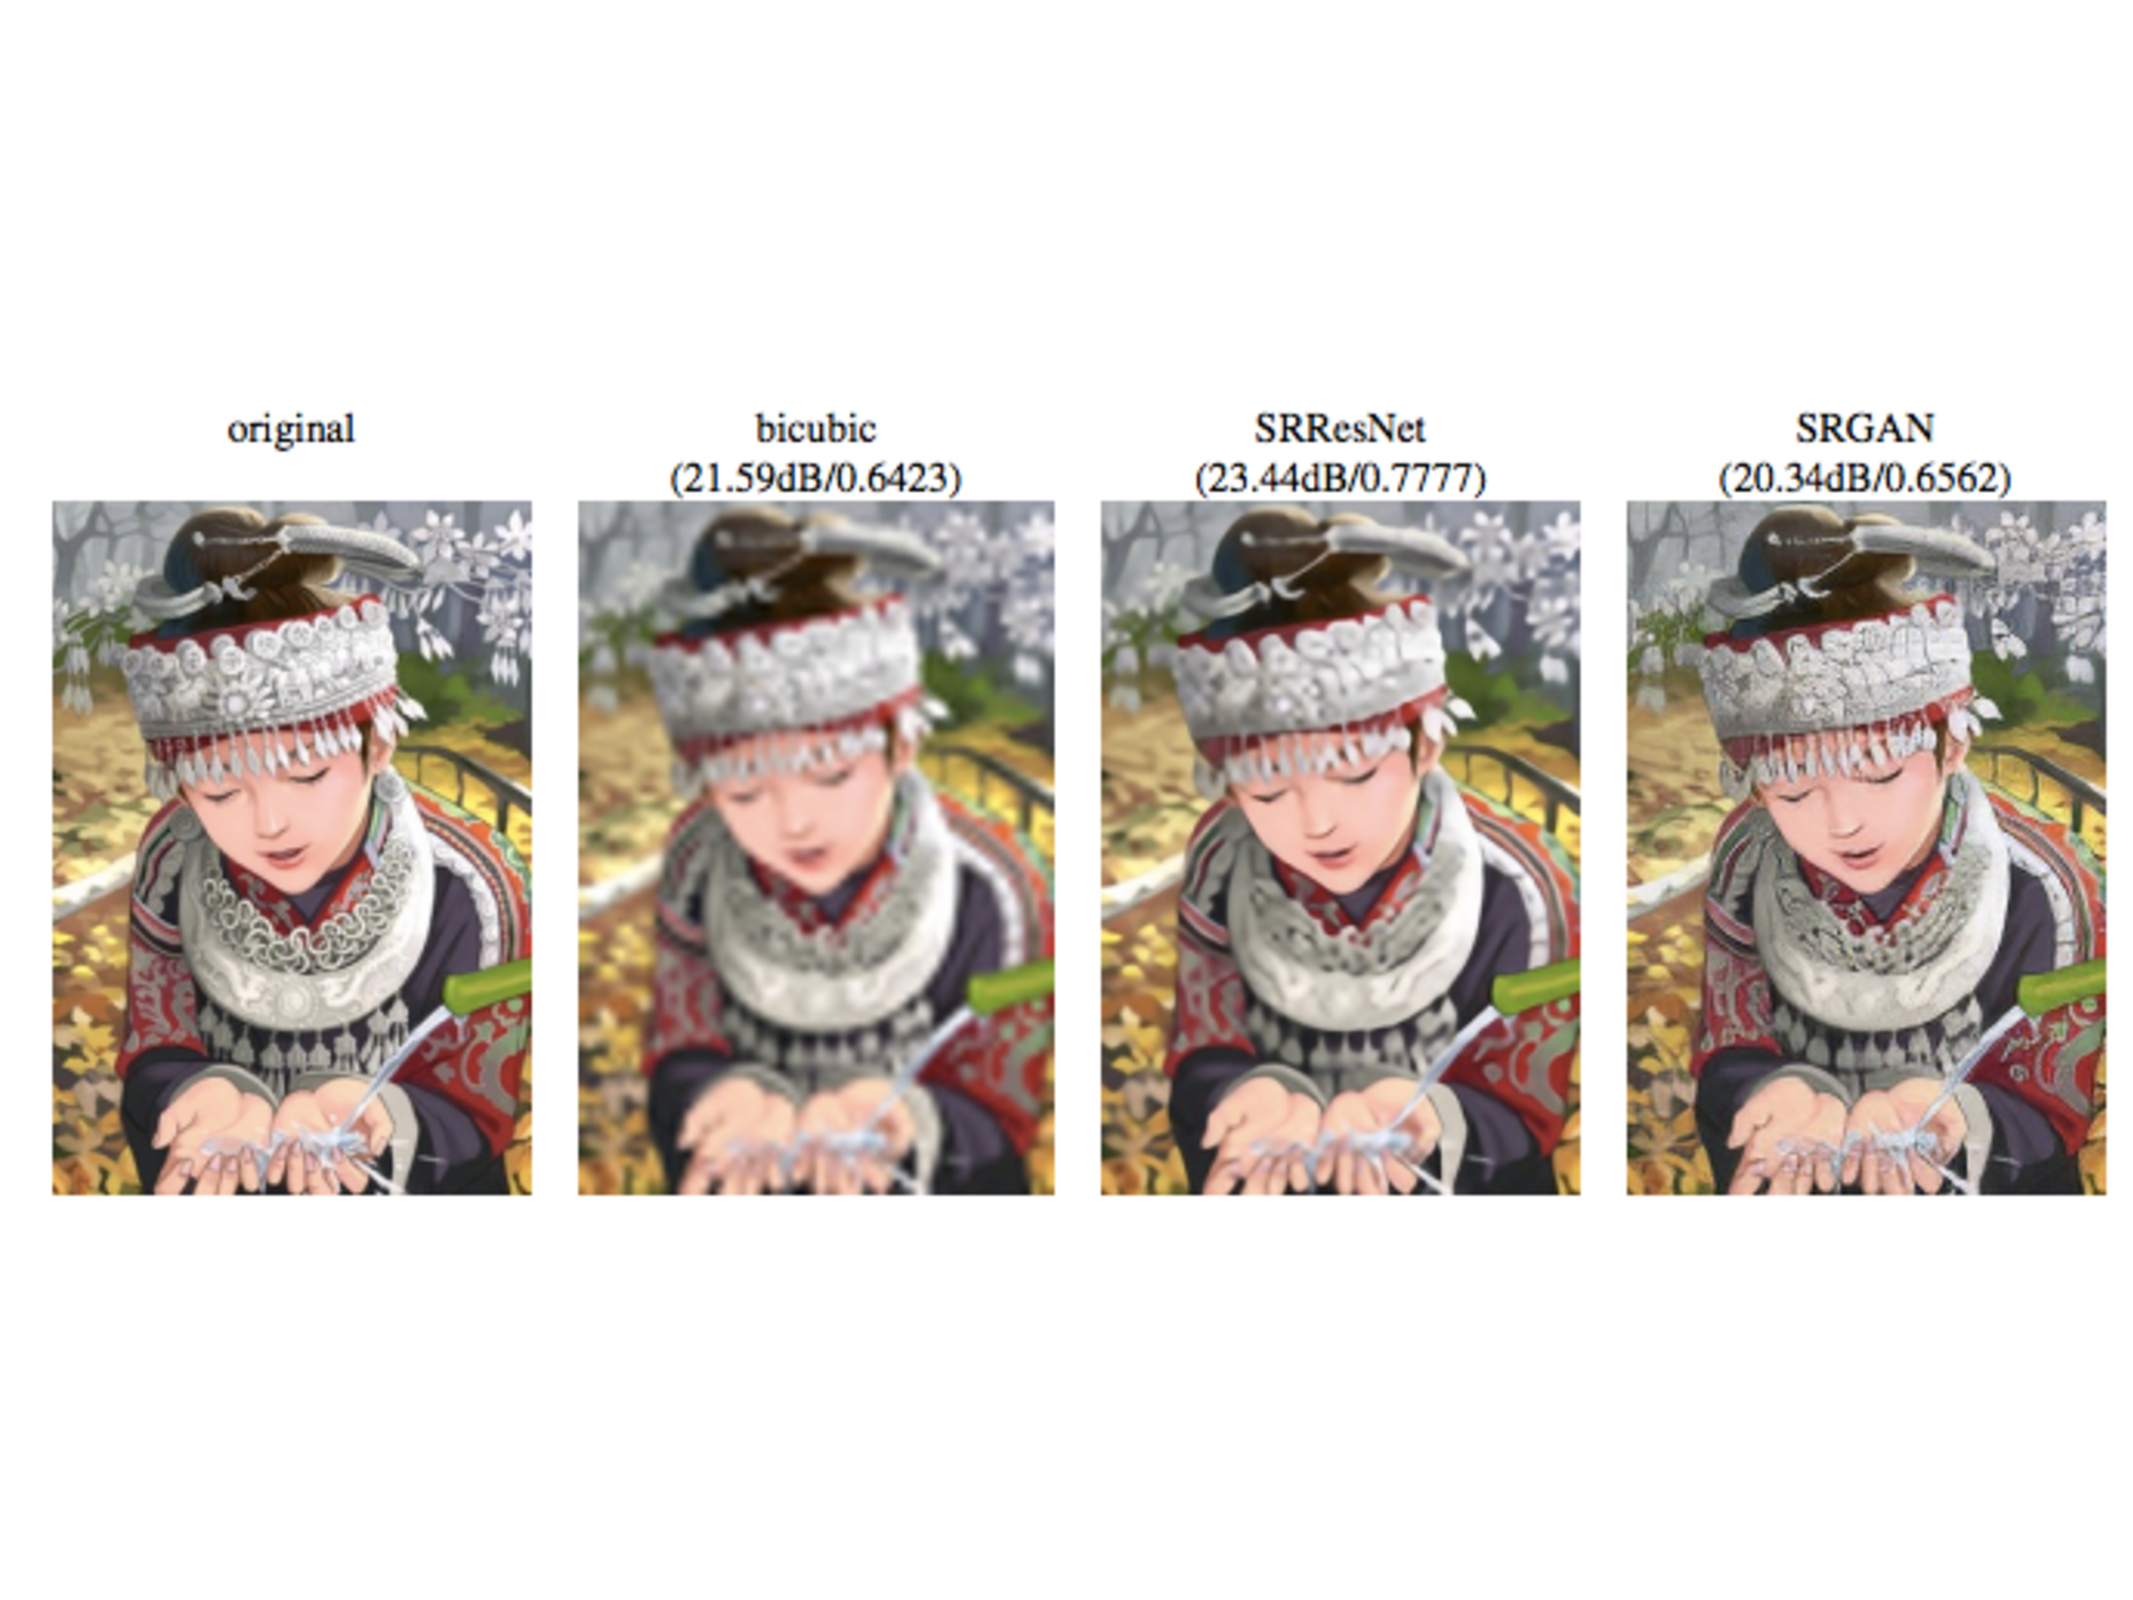
\includegraphics[width=\textwidth]{superres}
  \caption{
\citet{Ledig16} demonstrate excellent single-image superresolution results that show
the benefit of using a generative model trained to generate realistic samples from
 a multimodal distribution.
 The leftmost image is an original high-resolution image.
 It is then downsampled to make a low-resolution image, and different methods
 are used to attempt to recover the high-resolution image.
 The bicubic method is simply an interpolation method that does not use 
 the statistics of the training set at all.
 SRResNet is a neural network trained with mean squared error.
 SRGAN is a GAN-based neural network that improves over SRGAN because it is able
 to understand that there are multiple correct answers, rather than averaging
 over many answers to impose a single best output.
  }
  \label{fig:superres}
\end{figure}

\begin{figure}
  \centering
  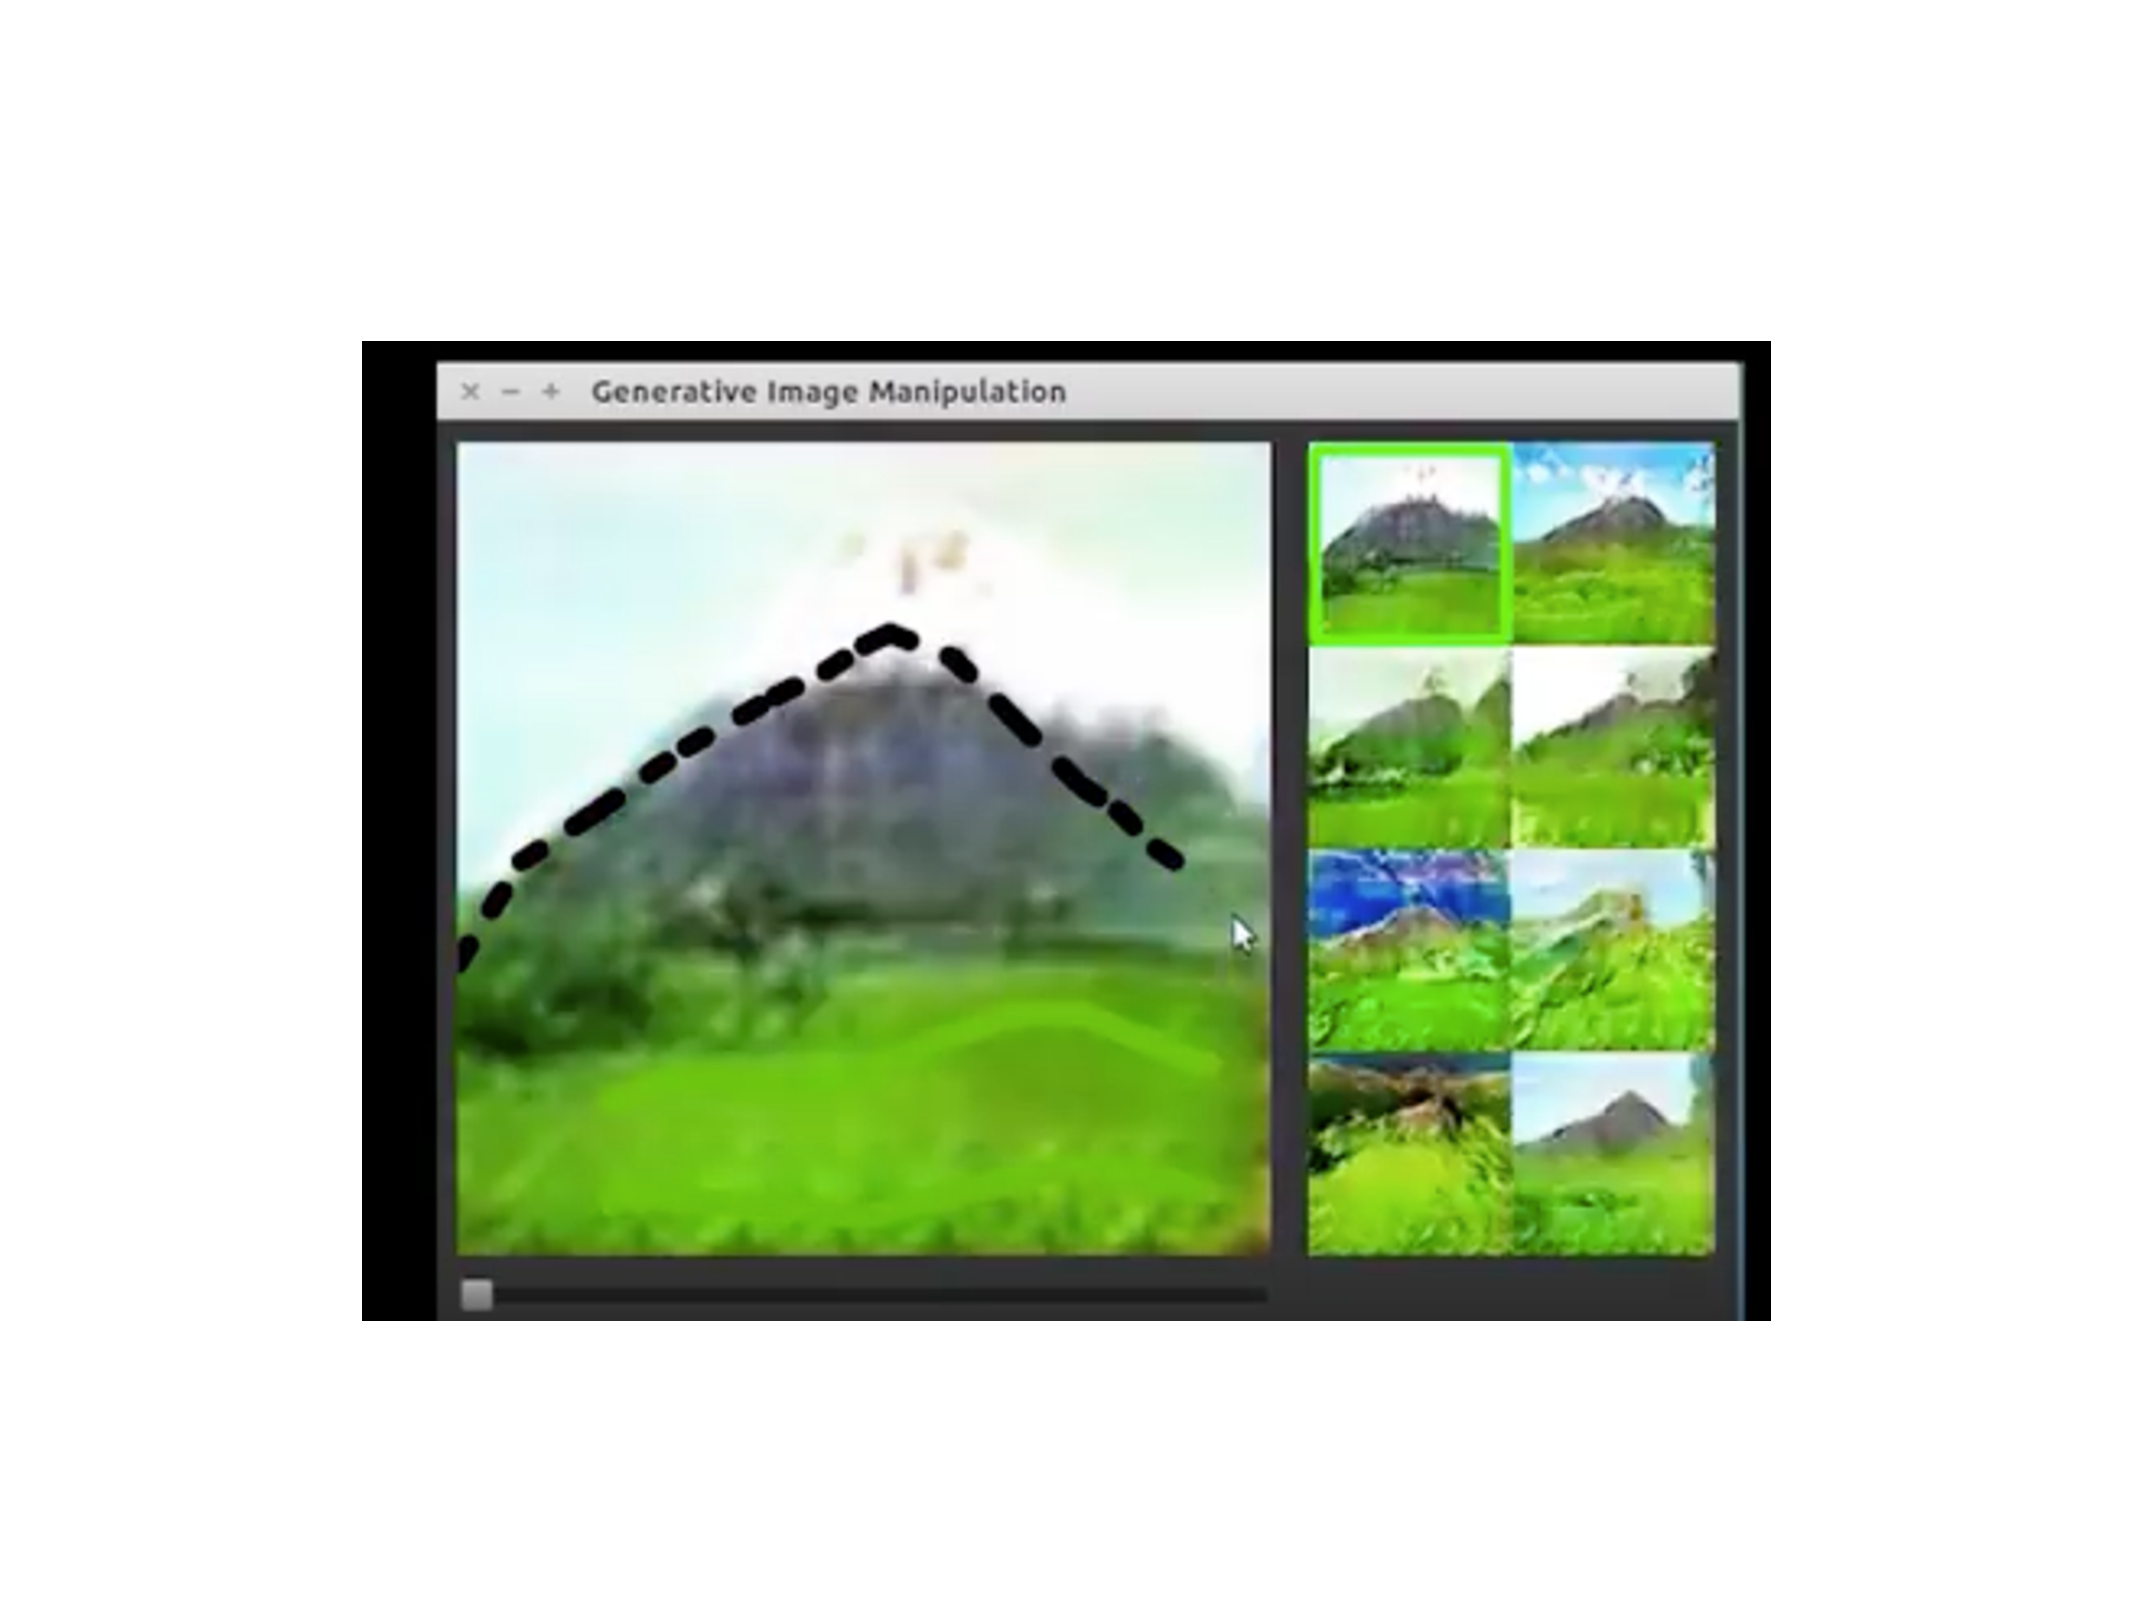
\includegraphics[width=\textwidth]{igan}
  \caption{
    \citet{zhu2016generative} developed an interactive application called {\em interactive generative adversarial networks}
(iGAN). 
A user can draw a rough sketch of an image, and iGAN uses a GAN to produce the most similar
realistic image.
In this example, a user has scribbled a few green lines that iGAN has converted into a grassy
field, and the user has drawn a black triangle that iGAN has turned into a detailed mountain.
Applications that create art are one of many reasons to study generative models that create
images.
A video demonstration of iGAN is available at the following URL:
\url{https://www.youtube.com/watch?v=9c4z6YsBGQ0}
}
  \label{fig:igan}
\end{figure}


\begin{figure}
  \centering
  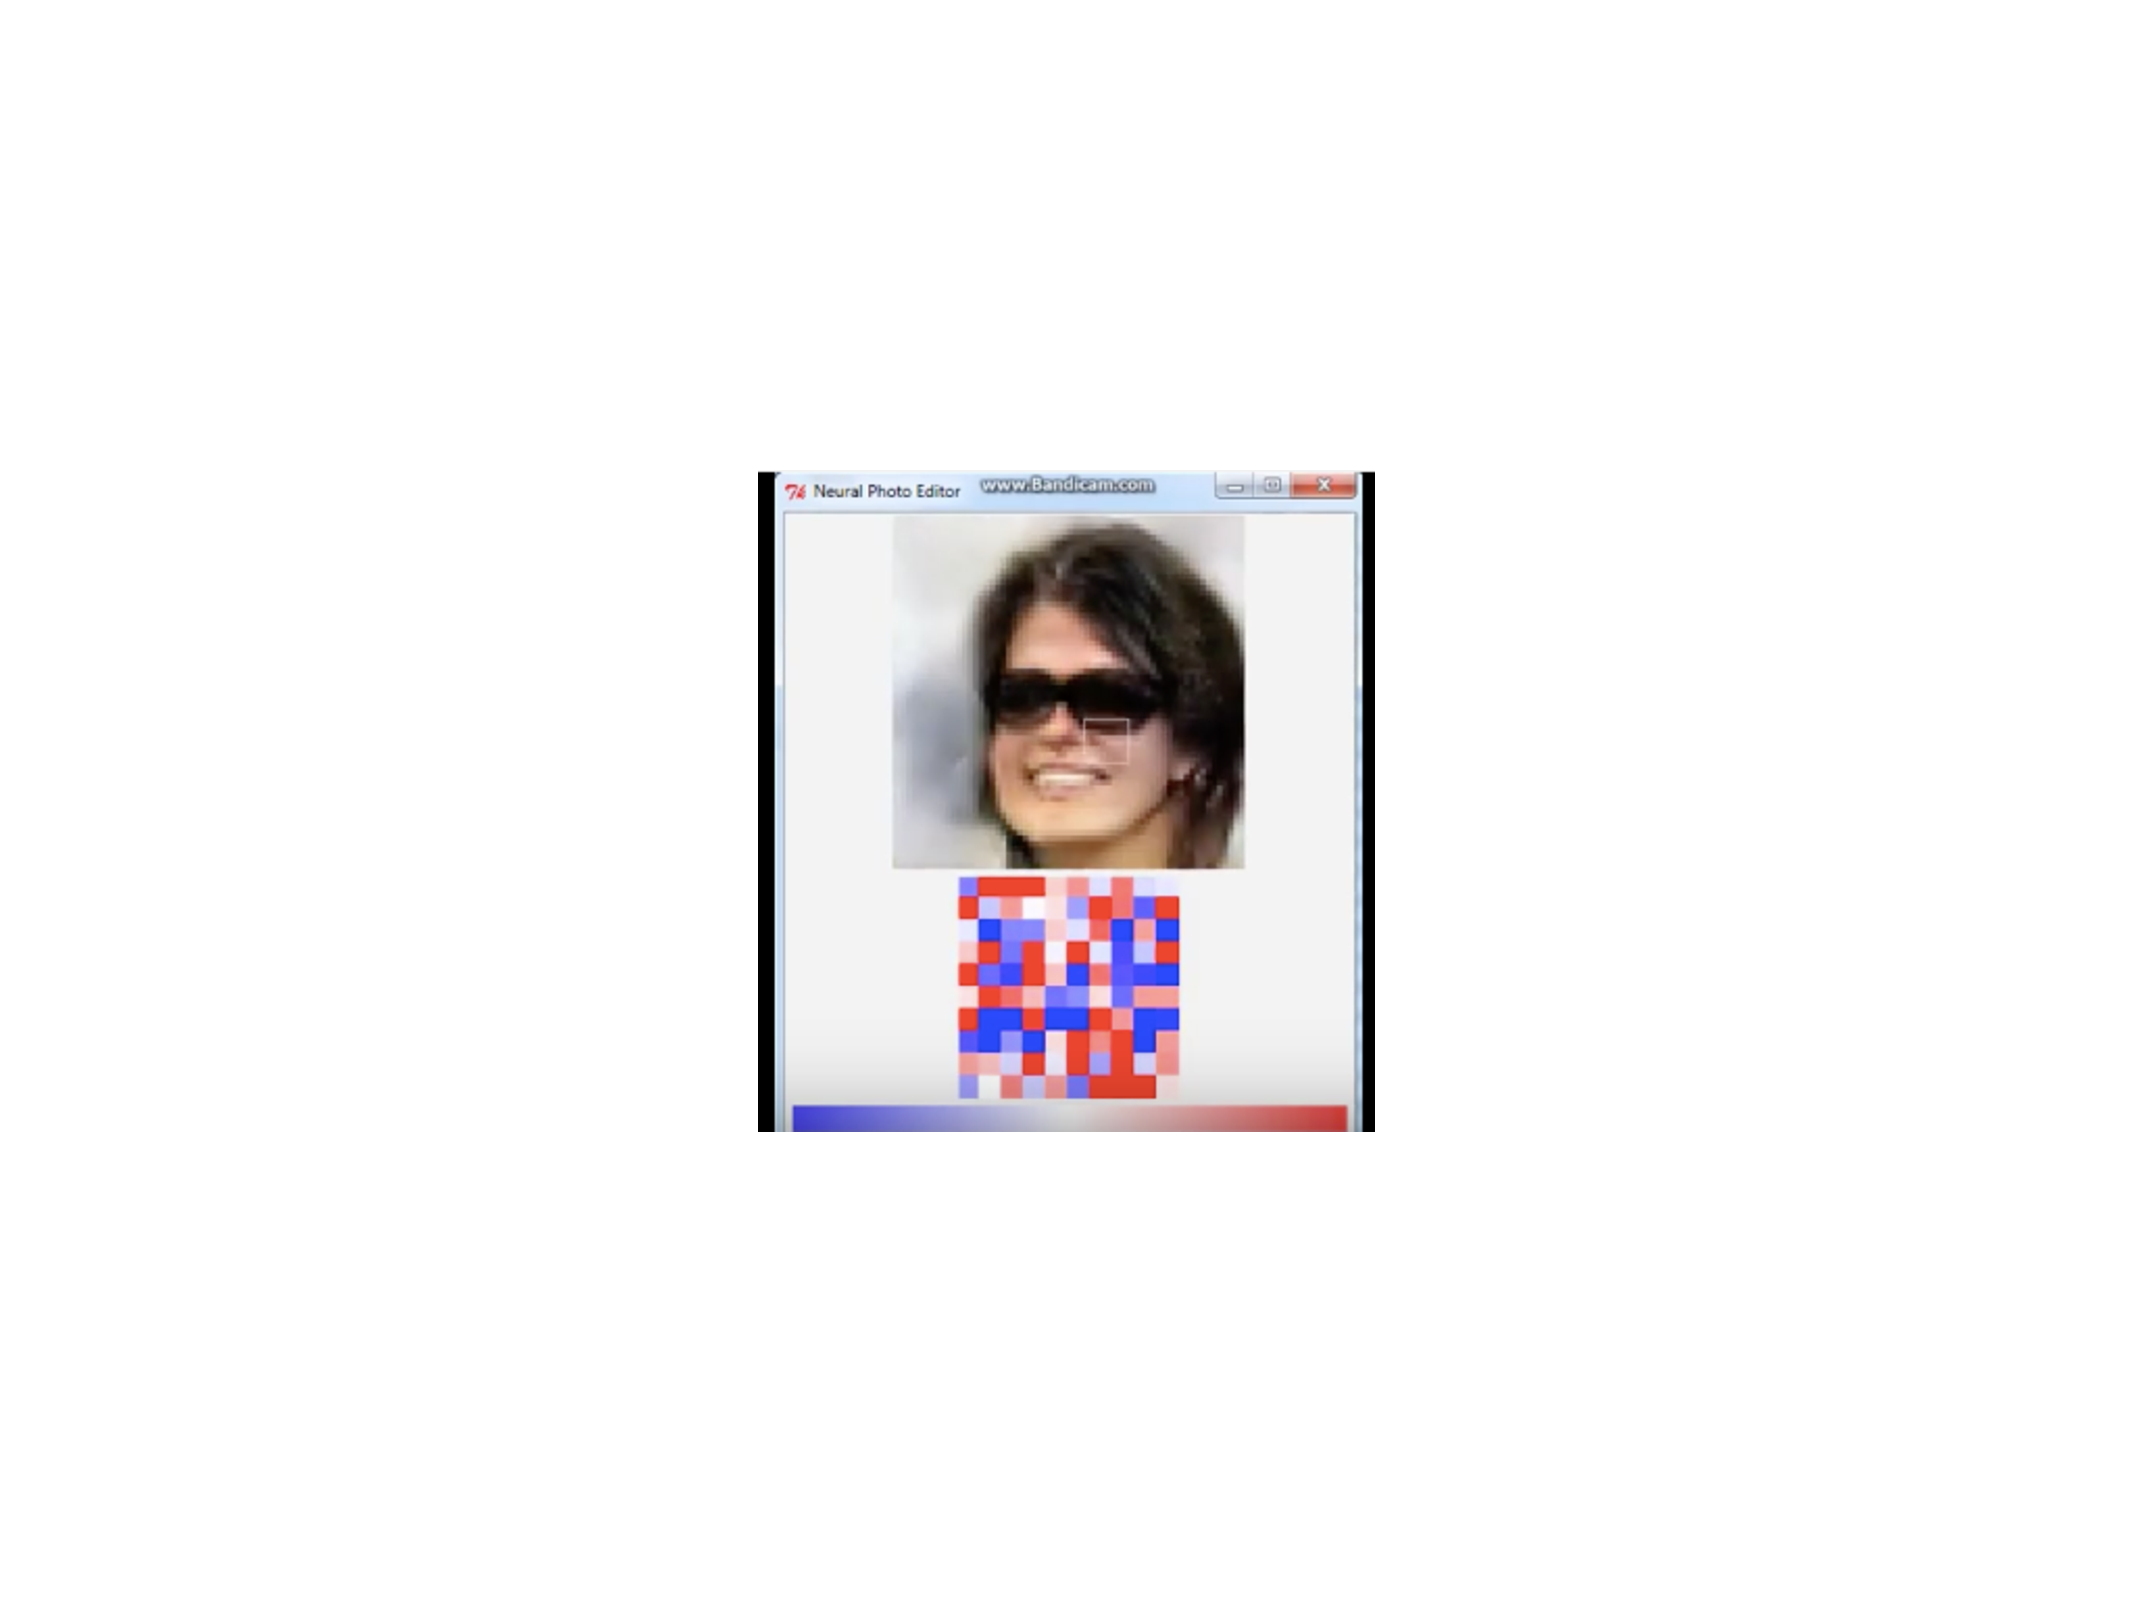
\includegraphics[width=\textwidth]{ian}
  \caption{
    \citet{BrockLRW16a} developed {\em introspective adversarial networks} (IAN).
    The user paints rough modifications to a photo, such as painting
    with black paint in an area where the user would like to add black
    hair, and IAN turns these rough paint strokes into photorealistic
    imagery matching the user's desires.
    Applications that enable a user to make realistic modifications to
    photo media are one of many reasons to study generative models
    that create images.
    A video demonstration of IAN is available at the following URL:
    \url{https://www.youtube.com/watch?v=FDELBFSeqQs}
  }
  \label{fig:ian}
\end{figure}

\begin{figure}
  \centering
  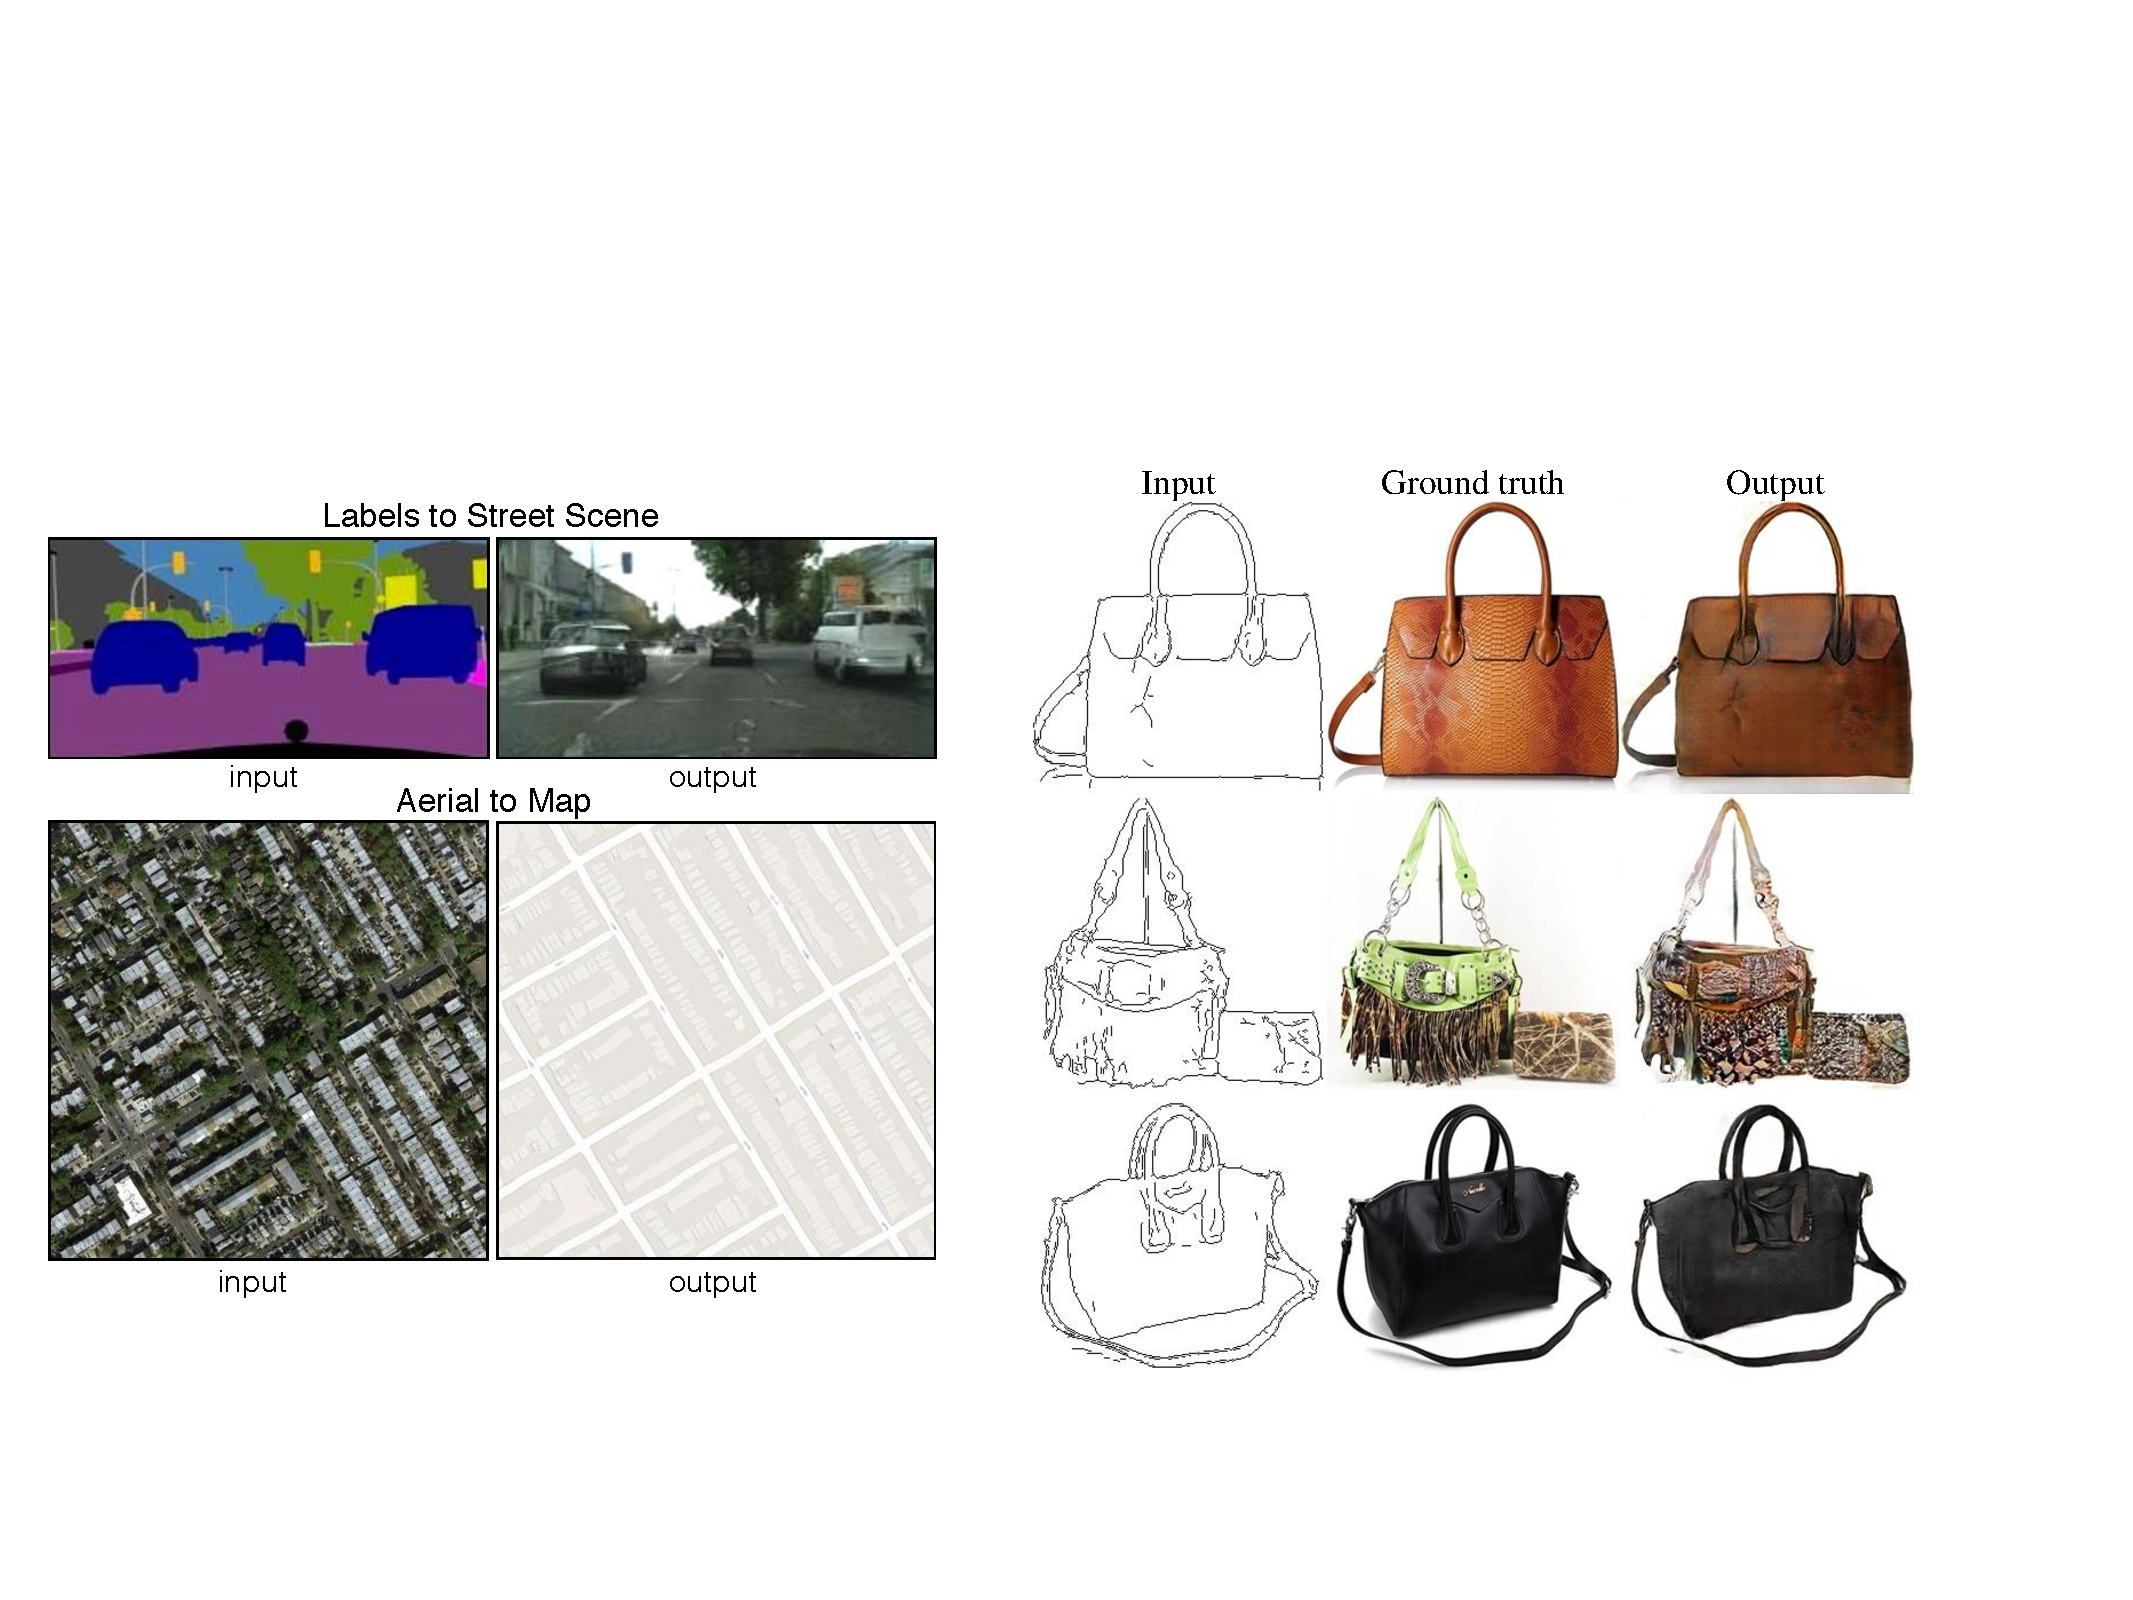
\includegraphics[width=\textwidth]{im2im}
  \caption{
    \citet{isola2016image}
    created a concept they called {image to image translation},
    encompassing many kinds of transformations of an image:
    converting a satellite photo into a map,
    coverting a sketch into a photorealistic image,
    etc.
    Because many of these conversion processes have multiple
    correct outputs for each input, it is necessary to use
    generative modeling to train the model correctly.
    In particular, \citet{isola2016image} use a GAN.
    Image to image translation provides many examples of how
    a creative algorithm designer can find several unanticipated uses
    for generative models.
    In the future, presumably many more such creative uses
    will be found.
  }
  \label{fig:im2im}
\end{figure}

All of these and other applications of generative models provide compelling
reasons to invest time and resources into improving generative models.

